% Options for packages loaded elsewhere
\PassOptionsToPackage{unicode}{hyperref}
\PassOptionsToPackage{hyphens}{url}
%
\documentclass[
]{article}
\usepackage{amsmath,amssymb}
\usepackage{iftex}
\ifPDFTeX
  \usepackage[T1]{fontenc}
  \usepackage[utf8]{inputenc}
  \usepackage{textcomp} % provide euro and other symbols
\else % if luatex or xetex
  \usepackage{unicode-math} % this also loads fontspec
  \defaultfontfeatures{Scale=MatchLowercase}
  \defaultfontfeatures[\rmfamily]{Ligatures=TeX,Scale=1}
\fi
\usepackage{lmodern}
\ifPDFTeX\else
  % xetex/luatex font selection
\fi
% Use upquote if available, for straight quotes in verbatim environments
\IfFileExists{upquote.sty}{\usepackage{upquote}}{}
\IfFileExists{microtype.sty}{% use microtype if available
  \usepackage[]{microtype}
  \UseMicrotypeSet[protrusion]{basicmath} % disable protrusion for tt fonts
}{}
\makeatletter
\@ifundefined{KOMAClassName}{% if non-KOMA class
  \IfFileExists{parskip.sty}{%
    \usepackage{parskip}
  }{% else
    \setlength{\parindent}{0pt}
    \setlength{\parskip}{6pt plus 2pt minus 1pt}}
}{% if KOMA class
  \KOMAoptions{parskip=half}}
\makeatother
\usepackage{xcolor}
\usepackage[margin=1in]{geometry}
\usepackage{graphicx}
\makeatletter
\def\maxwidth{\ifdim\Gin@nat@width>\linewidth\linewidth\else\Gin@nat@width\fi}
\def\maxheight{\ifdim\Gin@nat@height>\textheight\textheight\else\Gin@nat@height\fi}
\makeatother
% Scale images if necessary, so that they will not overflow the page
% margins by default, and it is still possible to overwrite the defaults
% using explicit options in \includegraphics[width, height, ...]{}
\setkeys{Gin}{width=\maxwidth,height=\maxheight,keepaspectratio}
% Set default figure placement to htbp
\makeatletter
\def\fps@figure{htbp}
\makeatother
\setlength{\emergencystretch}{3em} % prevent overfull lines
\providecommand{\tightlist}{%
  \setlength{\itemsep}{0pt}\setlength{\parskip}{0pt}}
\setcounter{secnumdepth}{5}
\newlength{\cslhangindent}
\setlength{\cslhangindent}{1.5em}
\newlength{\csllabelwidth}
\setlength{\csllabelwidth}{3em}
\newlength{\cslentryspacingunit} % times entry-spacing
\setlength{\cslentryspacingunit}{\parskip}
\newenvironment{CSLReferences}[2] % #1 hanging-ident, #2 entry spacing
 {% don't indent paragraphs
  \setlength{\parindent}{0pt}
  % turn on hanging indent if param 1 is 1
  \ifodd #1
  \let\oldpar\par
  \def\par{\hangindent=\cslhangindent\oldpar}
  \fi
  % set entry spacing
  \setlength{\parskip}{#2\cslentryspacingunit}
 }%
 {}
\usepackage{calc}
\newcommand{\CSLBlock}[1]{#1\hfill\break}
\newcommand{\CSLLeftMargin}[1]{\parbox[t]{\csllabelwidth}{#1}}
\newcommand{\CSLRightInline}[1]{\parbox[t]{\linewidth - \csllabelwidth}{#1}\break}
\newcommand{\CSLIndent}[1]{\hspace{\cslhangindent}#1}
\usepackage{float}
\usepackage{multirow}
\usepackage{lastpage}
\usepackage{fancyhdr}
\pagestyle{fancy}
\usepackage{booktabs}
\usepackage{longtable}
\usepackage{array}
\usepackage{multirow}
\usepackage{wrapfig}
\usepackage{float}
\usepackage{colortbl}
\usepackage{pdflscape}
\usepackage{tabu}
\usepackage{threeparttable}
\usepackage{threeparttablex}
\usepackage[normalem]{ulem}
\usepackage{makecell}
\usepackage{xcolor}
\ifLuaTeX
  \usepackage{selnolig}  % disable illegal ligatures
\fi
\IfFileExists{bookmark.sty}{\usepackage{bookmark}}{\usepackage{hyperref}}
\IfFileExists{xurl.sty}{\usepackage{xurl}}{} % add URL line breaks if available
\urlstyle{same}
\hypersetup{
  pdftitle={HCD Simulations Write Up},
  pdfauthor={Audrey Fu Lab},
  hidelinks,
  pdfcreator={LaTeX via pandoc}}

\title{HCD Simulations Write Up}
\author{Audrey Fu Lab}
\date{2024-03-07}

\begin{document}
\maketitle

\section*{Data Simulation}

\subsection*{Simulating the network}

We adopt a top-down approach to simulate hierarchical networks,
considering various simulation parameters such as graph sparsity, noise,
and the architecture of the super-level graph(s), including small-world,
scale-free, and random graph networks (Watts and Strogatz 1998; Barabási
and Bonabeau 2003).

Our simulations focus on basic hierarchies comprising one or two
hierarchical layers. Two-layer networks mirror classical community
detection on graphs, where our aim is to recover the true community
labels from a given graph. Meanwhile, three-layer networks present a
more intricate scenario, where the bottom layer of the hierarchy
contains two levels of community structure. Here, the top level
corresponds to the nodes at the uppermost layer of the hierarchy, and
the middle level consists of communities nested within the top-level
communities. The objective with these networks is to identify both sets
of community partitions.

In each hierarchy, for fully connected networks, we initiate by
simulating \(n_{\text{top}}\) top-level nodes, adhering to a directed
small-world, random graph, or scale-free network architecture (Watts and
Strogatz 1998; Barabási and Bonabeau 2003). In cases where the network
is disconnected, we simply simulate \(n_{\text{top}}\) disconnected
nodes. For networks with three hierarchical layers, we then generate a
subnetwork of \(n_{\text{middle}}\) nodes from each top-layer node,
adhering to the network structure utilized at the top level. If the
network is fully connected, we apply a probability \(p_\text{between}\)
to the nodes from different top-level communities being connected.

The final step in all hierarchies is to generate the nodes in the
observed (bottom) layer of the hierarchy. For each top-layer or
middle-layer node, we generate a subnetwork of \(n_{\text{bottom}}\)
nodes under the same subnetwork structure as the previous layers, and we
apply a probability \(p_\text{between}\) for nodes from different
communities to share an edge.

\subsection*{Simulating gene expression}

Once we simulate a hierarchical graph, we utilize this hierarchy to
generate the node-feature matrix, which depicts the expression of \(N\)
genes across \(p\) samples. Here, \(N\) denotes the number of nodes in
the observed (bottom) layer of the hierarchy, and its range is governed
by \(a^{\ell+1}<N<a\times b^\ell\), where \(\ell\) signifies the number
of hierarchical layers.

We simulate the node-feature matrix using the topological order the
observed level graph. We start by generating the features of nodes that
have no parental input. We refer to these nodes as origin nodes. All
origin nodes are simulated from a normal distribtion with mean \(0\) and
standard deviation \(\sigma\). All other nodes are simulated from a
normal distribution centered at the mean of their parent nodes and with
standard deviation \(\sigma\).

\section*{Datasets}

We consider three sets of hierarchical networks which represent varying
difficulty levels for inference:

\begin{itemize}
  \item[1.] \textbf{Complex networks} - - used for final simulation assessment - \textbf{Table 1-3}
  \item[2.] \textbf{Intermediate networks} - used for investigative model tuning and performance assessment - \textbf{Table 4}
  \item[3.] \textbf{Simple networks} - used for code implementation and debugging - \textbf{Table 5}
\end{itemize}

\section*{Application to Intermediate Networks}

A summary of the intermediate networks can be found in \textbf{Table 4}.
The intermediate networks dataset consists of three layer networks of
small world, scale free, and random graph architectures that are less
complex then the three layer networks in the \textbf{Complex networks}
dataset. Each of these networks has \(5\) super layer nodes, \(15\)
middle layer nodes and approximately \(300\) bottom layer nodes. We
primarily use this dataset to investigate the behavior of the HCD method
when applied to 3-layer network.

\section*{Preliminary Findings}

\newpage

\section*{Tables}

\begin{table}
\centering\centering
\caption{\label{tab:unnamed-chunk-1}Summary statistics for all small world networks in the complex networks datset}
\centering
\fontsize{10}{12}\selectfont
\fontsize{9}{11}\selectfont
\begin{tabular}[t]{>{\raggedright\arraybackslash}p{6em}>{\raggedright\arraybackslash}p{4em}>{\raggedright\arraybackslash}p{4em}>{\raggedright\arraybackslash}p{4em}>{\raggedright\arraybackslash}p{4em}>{\raggedright\arraybackslash}p{4em}>{\raggedright\arraybackslash}p{4em}>{\raggedright\arraybackslash}p{4em}>{\raggedright\arraybackslash}p{4em}}
\toprule
Value & Network1 & Network2 & Network3 & Network4 & Network5 & Network6 & Network7 & Network8\\
\midrule
\cellcolor{gray!10}{Subgraph type} & \cellcolor{gray!10}{small world} & \cellcolor{gray!10}{small world} & \cellcolor{gray!10}{small world} & \cellcolor{gray!10}{small world} & \cellcolor{gray!10}{small world} & \cellcolor{gray!10}{small world} & \cellcolor{gray!10}{small world} & \cellcolor{gray!10}{small world}\\
Connection type & disc & disc & disc & disc & full & full & full & full\\
\cellcolor{gray!10}{Layers} & \cellcolor{gray!10}{2} & \cellcolor{gray!10}{2} & \cellcolor{gray!10}{3} & \cellcolor{gray!10}{3} & \cellcolor{gray!10}{2} & \cellcolor{gray!10}{2} & \cellcolor{gray!10}{3} & \cellcolor{gray!10}{3}\\
Standard deviation & 0.1 & 0.5 & 0.1 & 0.5 & 0.1 & 0.5 & 0.1 & 0.5\\
\cellcolor{gray!10}{Nodes per layer} & \cellcolor{gray!10}{(10, 63)} & \cellcolor{gray!10}{(10, 63)} & \cellcolor{gray!10}{(10, 63, 1604)} & \cellcolor{gray!10}{(10, 63, 1604)} & \cellcolor{gray!10}{(10, 63)} & \cellcolor{gray!10}{(10, 63)} & \cellcolor{gray!10}{(10, 63, 1604)} & \cellcolor{gray!10}{(10, 63, 1604)}\\
\addlinespace
Edges per layer & (0, 63) & (0, 63) & (0, 63, 2011) & (0, 63, 2031) & (45, 115) & (45, 109) & (45, 114, 1604) & (45, 111, 1604)\\
\cellcolor{gray!10}{Subgraph probability} & \cellcolor{gray!10}{0.05} & \cellcolor{gray!10}{0.05} & \cellcolor{gray!10}{0.05} & \cellcolor{gray!10}{0.05} & \cellcolor{gray!10}{0.05} & \cellcolor{gray!10}{0.05} & \cellcolor{gray!10}{0.05} & \cellcolor{gray!10}{0.05}\\
Sample size & 500 & 500 & 500 & 500 & 500 & 500 & 500 & 500\\
\cellcolor{gray!10}{Modularity (top)} & \cellcolor{gray!10}{0.898} & \cellcolor{gray!10}{0.898} & \cellcolor{gray!10}{0.898} & \cellcolor{gray!10}{0.898} & \cellcolor{gray!10}{0.447} & \cellcolor{gray!10}{0.477} & \cellcolor{gray!10}{0.766} & \cellcolor{gray!10}{0.771}\\
Average node degree top & 1 & 1 & 1.254 & 1.266 & 1.825 & 1.73 & 1.433 & 1.439\\
\addlinespace
\cellcolor{gray!10}{Avg connections within top communities} & \cellcolor{gray!10}{6.3} & \cellcolor{gray!10}{6.3} & \cellcolor{gray!10}{201.1} & \cellcolor{gray!10}{203.1} & \cellcolor{gray!10}{6.3} & \cellcolor{gray!10}{6.3} & \cellcolor{gray!10}{199.3} & \cellcolor{gray!10}{201.3}\\
Avg. connections between top communities & 0 & 0 & 0 & 0 & 0.578 & 0.511 & 3.389 & 3.278\\
\cellcolor{gray!10}{Modularity (middle)} & \cellcolor{gray!10}{NA} & \cellcolor{gray!10}{NA} & \cellcolor{gray!10}{0.762} & \cellcolor{gray!10}{0.758} & \cellcolor{gray!10}{NA} & \cellcolor{gray!10}{NA} & \cellcolor{gray!10}{0.667} & \cellcolor{gray!10}{0.663}\\
Average node degree middle & NA & NA & 1.254 & 1.266 & NA & NA & 1.433 & 1.439\\
\cellcolor{gray!10}{Avg connections within middle communities} & \cellcolor{gray!10}{NA} & \cellcolor{gray!10}{NA} & \cellcolor{gray!10}{24.825} & \cellcolor{gray!10}{24.968} & \cellcolor{gray!10}{NA} & \cellcolor{gray!10}{NA} & \cellcolor{gray!10}{24.937} & \cellcolor{gray!10}{24.873}\\
\addlinespace
Avg connections between middle communities & NA & NA & 0.114 & 0.117 & NA & NA & 0.186 & 0.19\\
\bottomrule
\end{tabular}
\end{table}

\begin{table}
\centering\centering
\caption{\label{tab:unnamed-chunk-2}Summary statistics for all scale free networks in the complex networks datset}
\centering
\fontsize{10}{12}\selectfont
\fontsize{9}{11}\selectfont
\begin{tabular}[t]{>{\raggedright\arraybackslash}p{6em}>{\raggedright\arraybackslash}p{4em}>{\raggedright\arraybackslash}p{4em}>{\raggedright\arraybackslash}p{4em}>{\raggedright\arraybackslash}p{4em}>{\raggedright\arraybackslash}p{4em}>{\raggedright\arraybackslash}p{4em}>{\raggedright\arraybackslash}p{4em}>{\raggedright\arraybackslash}p{4em}}
\toprule
Value & Network1 & Network2 & Network3 & Network4 & Network5 & Network6 & Network7 & Network8\\
\midrule
\cellcolor{gray!10}{Subgraph type} & \cellcolor{gray!10}{scale free} & \cellcolor{gray!10}{scale free} & \cellcolor{gray!10}{scale free} & \cellcolor{gray!10}{scale free} & \cellcolor{gray!10}{scale free} & \cellcolor{gray!10}{scale free} & \cellcolor{gray!10}{scale free} & \cellcolor{gray!10}{scale free}\\
Connection type & disc & disc & disc & disc & full & full & full & full\\
\cellcolor{gray!10}{Layers} & \cellcolor{gray!10}{2} & \cellcolor{gray!10}{2} & \cellcolor{gray!10}{3} & \cellcolor{gray!10}{3} & \cellcolor{gray!10}{2} & \cellcolor{gray!10}{2} & \cellcolor{gray!10}{3} & \cellcolor{gray!10}{3}\\
Standard deviation & 0.1 & 0.5 & 0.1 & 0.5 & 0.1 & 0.5 & 0.1 & 0.5\\
\cellcolor{gray!10}{Nodes per layer} & \cellcolor{gray!10}{(10, 58)} & \cellcolor{gray!10}{(10, 58)} & \cellcolor{gray!10}{(10, 58, 1450)} & \cellcolor{gray!10}{(10, 58, 1450)} & \cellcolor{gray!10}{(10, 58)} & \cellcolor{gray!10}{(10, 58)} & \cellcolor{gray!10}{(10, 58, 1450)} & \cellcolor{gray!10}{(10, 58, 1450)}\\
\addlinespace
Edges per layer & (0, 74) & (0, 74) & (0, 74, 6700) & (0, 74, 6670) & (45, 120) & (45, 120) & (45, 123, 1450) & (45, 122, 1450)\\
\cellcolor{gray!10}{Subgraph probability} & \cellcolor{gray!10}{0.05} & \cellcolor{gray!10}{0.05} & \cellcolor{gray!10}{0.05} & \cellcolor{gray!10}{0.05} & \cellcolor{gray!10}{0.05} & \cellcolor{gray!10}{0.05} & \cellcolor{gray!10}{0.05} & \cellcolor{gray!10}{0.05}\\
Sample size & 500 & 500 & 500 & 500 & 500 & 500 & 500 & 500\\
\cellcolor{gray!10}{Modularity (top)} & \cellcolor{gray!10}{0.89} & \cellcolor{gray!10}{0.89} & \cellcolor{gray!10}{0.892} & \cellcolor{gray!10}{0.893} & \cellcolor{gray!10}{0.513} & \cellcolor{gray!10}{0.513} & \cellcolor{gray!10}{0.854} & \cellcolor{gray!10}{0.849}\\
Average node degree top & 1.276 & 1.276 & 4.621 & 4.6 & 2.069 & 2.069 & 4.781 & 4.843\\
\addlinespace
\cellcolor{gray!10}{Avg connections within top communities} & \cellcolor{gray!10}{7.4} & \cellcolor{gray!10}{7.4} & \cellcolor{gray!10}{670} & \cellcolor{gray!10}{667} & \cellcolor{gray!10}{7.4} & \cellcolor{gray!10}{7.4} & \cellcolor{gray!10}{665.9} & \cellcolor{gray!10}{671.4}\\
Avg. connections between top communities & 0 & 0 & 0 & 0 & 0.511 & 0.511 & 3.033 & 3.422\\
\cellcolor{gray!10}{Modularity (middle)} & \cellcolor{gray!10}{NA} & \cellcolor{gray!10}{NA} & \cellcolor{gray!10}{0.906} & \cellcolor{gray!10}{0.91} & \cellcolor{gray!10}{NA} & \cellcolor{gray!10}{NA} & \cellcolor{gray!10}{0.875} & \cellcolor{gray!10}{0.864}\\
Average node degree middle & NA & NA & 4.621 & 4.6 & NA & NA & 4.781 & 4.843\\
\cellcolor{gray!10}{Avg connections within middle communities} & \cellcolor{gray!10}{NA} & \cellcolor{gray!10}{NA} & \cellcolor{gray!10}{107.069} & \cellcolor{gray!10}{107.069} & \cellcolor{gray!10}{NA} & \cellcolor{gray!10}{NA} & \cellcolor{gray!10}{107.069} & \cellcolor{gray!10}{107.069}\\
\addlinespace
Avg connections between middle communities & NA & NA & 0.148 & 0.139 & NA & NA & 0.218 & 0.246\\
\bottomrule
\end{tabular}
\end{table}

\begin{table}
\centering\centering
\caption{\label{tab:unnamed-chunk-3}Summary statistics for all random graph networks in the complex networks datset}
\centering
\fontsize{10}{12}\selectfont
\fontsize{9}{11}\selectfont
\begin{tabular}[t]{>{\raggedright\arraybackslash}p{6em}>{\raggedright\arraybackslash}p{4em}>{\raggedright\arraybackslash}p{4em}>{\raggedright\arraybackslash}p{4em}>{\raggedright\arraybackslash}p{4em}>{\raggedright\arraybackslash}p{4em}>{\raggedright\arraybackslash}p{4em}>{\raggedright\arraybackslash}p{4em}>{\raggedright\arraybackslash}p{4em}}
\toprule
Value & Network1 & Network2 & Network3 & Network4 & Network5 & Network6 & Network7 & Network8\\
\midrule
\cellcolor{gray!10}{Subgraph type} & \cellcolor{gray!10}{random graph} & \cellcolor{gray!10}{random graph} & \cellcolor{gray!10}{random graph} & \cellcolor{gray!10}{random graph} & \cellcolor{gray!10}{random graph} & \cellcolor{gray!10}{random graph} & \cellcolor{gray!10}{random graph} & \cellcolor{gray!10}{random graph}\\
Connection type & disc & disc & disc & disc & full & full & full & full\\
\cellcolor{gray!10}{Layers} & \cellcolor{gray!10}{2} & \cellcolor{gray!10}{2} & \cellcolor{gray!10}{3} & \cellcolor{gray!10}{3} & \cellcolor{gray!10}{2} & \cellcolor{gray!10}{2} & \cellcolor{gray!10}{3} & \cellcolor{gray!10}{3}\\
Standard deviation & 0.1 & 0.5 & 0.1 & 0.5 & 0.1 & 0.5 & 0.1 & 0.5\\
\cellcolor{gray!10}{Nodes per layer} & \cellcolor{gray!10}{(10, 45)} & \cellcolor{gray!10}{(10, 45)} & \cellcolor{gray!10}{(10, 45, 725)} & \cellcolor{gray!10}{(10, 45, 725)} & \cellcolor{gray!10}{(10, 45)} & \cellcolor{gray!10}{(10, 45)} & \cellcolor{gray!10}{(10, 45, 725)} & \cellcolor{gray!10}{(10, 45, 725)}\\
\addlinespace
Edges per layer & (0, 32) & (0, 32) & (0, 32, 678) & (0, 32, 665) & (45, 77) & (45, 77) & (45, 78, 725) & (45, 78, 725)\\
\cellcolor{gray!10}{Subgraph probability} & \cellcolor{gray!10}{0.05} & \cellcolor{gray!10}{0.05} & \cellcolor{gray!10}{0.05} & \cellcolor{gray!10}{0.05} & \cellcolor{gray!10}{0.05} & \cellcolor{gray!10}{0.05} & \cellcolor{gray!10}{0.05} & \cellcolor{gray!10}{0.05}\\
Sample size & 500 & 500 & 500 & 500 & 500 & 500 & 500 & 500\\
\cellcolor{gray!10}{Modularity (top)} & \cellcolor{gray!10}{0.883} & \cellcolor{gray!10}{0.883} & \cellcolor{gray!10}{0.886} & \cellcolor{gray!10}{0.885} & \cellcolor{gray!10}{0.313} & \cellcolor{gray!10}{0.313} & \cellcolor{gray!10}{0.758} & \cellcolor{gray!10}{0.721}\\
Average node degree top & 0.711 & 0.711 & 0.935 & 0.917 & 1.711 & 1.711 & 1.04 & 1.09\\
\addlinespace
\cellcolor{gray!10}{Avg connections within top communities} & \cellcolor{gray!10}{3.2} & \cellcolor{gray!10}{3.2} & \cellcolor{gray!10}{67.8} & \cellcolor{gray!10}{66.5} & \cellcolor{gray!10}{3.2} & \cellcolor{gray!10}{3.2} & \cellcolor{gray!10}{65.5} & \cellcolor{gray!10}{65.7}\\
Avg. connections between top communities & 0 & 0 & 0 & 0 & 0.5 & 0.5 & 1.1 & 1.478\\
\cellcolor{gray!10}{Modularity (middle)} & \cellcolor{gray!10}{NA} & \cellcolor{gray!10}{NA} & \cellcolor{gray!10}{0.783} & \cellcolor{gray!10}{0.803} & \cellcolor{gray!10}{NA} & \cellcolor{gray!10}{NA} & \cellcolor{gray!10}{0.703} & \cellcolor{gray!10}{0.669}\\
Average node degree middle & NA & NA & 0.935 & 0.917 & NA & NA & 1.04 & 1.09\\
\cellcolor{gray!10}{Avg connections within middle communities} & \cellcolor{gray!10}{NA} & \cellcolor{gray!10}{NA} & \cellcolor{gray!10}{12.156} & \cellcolor{gray!10}{12.222} & \cellcolor{gray!10}{NA} & \cellcolor{gray!10}{NA} & \cellcolor{gray!10}{12.178} & \cellcolor{gray!10}{12.156}\\
\addlinespace
Avg connections between middle communities & NA & NA & 0.066 & 0.058 & NA & NA & 0.104 & 0.123\\
\bottomrule
\end{tabular}
\end{table}

\clearpage
\newpage
\begin{table}
\centering\centering
\caption{\label{tab:unnamed-chunk-4}Summary statistics for intermediate difficulty simulated networks.}
\centering
\fontsize{10}{12}\selectfont
\fontsize{10}{12}\selectfont
\begin{tabular}[t]{>{\raggedright\arraybackslash}p{8em}llllll}
\toprule
Value & Network1 & Network2 & Network3 & Network4 & Network5 & Network6\\
\midrule
\cellcolor{gray!10}{Subgraph type} & \cellcolor{gray!10}{small world} & \cellcolor{gray!10}{small world} & \cellcolor{gray!10}{scale free} & \cellcolor{gray!10}{scale free} & \cellcolor{gray!10}{random graph} & \cellcolor{gray!10}{random graph}\\
Connection type & disc & full & disc & full & disc & full\\
\cellcolor{gray!10}{Layers} & \cellcolor{gray!10}{3} & \cellcolor{gray!10}{3} & \cellcolor{gray!10}{3} & \cellcolor{gray!10}{3} & \cellcolor{gray!10}{3} & \cellcolor{gray!10}{3}\\
Standard deviation & 0.1 & 0.1 & 0.1 & 0.1 & 0.1 & 0.1\\
\cellcolor{gray!10}{Nodes per layer} & \cellcolor{gray!10}{(5, 15, 300)} & \cellcolor{gray!10}{(5, 15, 300)} & \cellcolor{gray!10}{(5, 15, 300)} & \cellcolor{gray!10}{(5, 15, 300)} & \cellcolor{gray!10}{(5, 12, 167)} & \cellcolor{gray!10}{(5, 12, 167)}\\
\addlinespace
Edges per layer & (0, 15, 354) & (10, 25, 300) & (0, 10, 966) & (10, 20, 300) & (0, 7, 133) & (10, 17, 167)\\
\cellcolor{gray!10}{Subgraph probability} & \cellcolor{gray!10}{0.05} & \cellcolor{gray!10}{0.05} & \cellcolor{gray!10}{0.05} & \cellcolor{gray!10}{0.05} & \cellcolor{gray!10}{0.05} & \cellcolor{gray!10}{0.05}\\
Sample size & 500 & 500 & 500 & 500 & 500 & 500\\
\cellcolor{gray!10}{Modularity (top)} & \cellcolor{gray!10}{0.799} & \cellcolor{gray!10}{0.715} & \cellcolor{gray!10}{0.78} & \cellcolor{gray!10}{0.751} & \cellcolor{gray!10}{0.791} & \cellcolor{gray!10}{0.665}\\
Average node degree top & 1.18 & 1.34 & 3.22 & 3.32 & 0.796 & 0.886\\
\addlinespace
\cellcolor{gray!10}{Avg connections within top communities} & \cellcolor{gray!10}{70.8} & \cellcolor{gray!10}{73.6} & \cellcolor{gray!10}{193.2} & \cellcolor{gray!10}{193.2} & \cellcolor{gray!10}{26.6} & \cellcolor{gray!10}{26}\\
Avg. connections between top communities & 0 & 1.7 & 0 & 1.5 & 0 & 0.9\\
\cellcolor{gray!10}{Modularity (middle)} & \cellcolor{gray!10}{0.781} & \cellcolor{gray!10}{0.679} & \cellcolor{gray!10}{0.873} & \cellcolor{gray!10}{0.845} & \cellcolor{gray!10}{0.787} & \cellcolor{gray!10}{0.696}\\
Average node degree middle & 1.18 & 1.34 & 3.22 & 3.32 & 0.796 & 0.886\\
\cellcolor{gray!10}{Avg connections within middle communities} & \cellcolor{gray!10}{20} & \cellcolor{gray!10}{20} & \cellcolor{gray!10}{61.333} & \cellcolor{gray!10}{61.333} & \cellcolor{gray!10}{9.667} & \cellcolor{gray!10}{9.667}\\
\addlinespace
Avg connections between middle communities & 0.257 & 0.486 & 0.219 & 0.362 & 0.129 & 0.242\\
\bottomrule
\end{tabular}
\end{table}

\begin{table}
\centering\centering
\caption{\label{tab:unnamed-chunk-5}Summary statistics for simple simulated networks. These networks contain fewer than 100 nodes at the observed level and only cover small world subgraph architecture}
\centering
\fontsize{10}{12}\selectfont
\fontsize{10}{12}\selectfont
\begin{tabular}[t]{>{\raggedright\arraybackslash}p{8em}llll}
\toprule
Value & Network1 & Network2 & Network3 & Network4\\
\midrule
\cellcolor{gray!10}{Subgraph type} & \cellcolor{gray!10}{small world} & \cellcolor{gray!10}{small world} & \cellcolor{gray!10}{small world} & \cellcolor{gray!10}{small world}\\
Connection type & disc & disc & full & full\\
\cellcolor{gray!10}{Layers} & \cellcolor{gray!10}{2} & \cellcolor{gray!10}{3} & \cellcolor{gray!10}{2} & \cellcolor{gray!10}{3}\\
Standard deviation & 0.1 & 0.1 & 0.1 & 0.1\\
\cellcolor{gray!10}{Nodes per layer} & \cellcolor{gray!10}{(2, 6)} & \cellcolor{gray!10}{(2, 6, 18)} & \cellcolor{gray!10}{(2, 6)} & \cellcolor{gray!10}{(2, 6, 18)}\\
\addlinespace
Edges per layer & (0, 6) & (0, 6, 24) & (1, 7) & (1, 7, 18)\\
\cellcolor{gray!10}{Subgraph probability} & \cellcolor{gray!10}{0.05} & \cellcolor{gray!10}{0.05} & \cellcolor{gray!10}{0.05} & \cellcolor{gray!10}{0.05}\\
Sample size & 500 & 500 & 500 & 500\\
\cellcolor{gray!10}{Modularity (top)} & \cellcolor{gray!10}{0.5} & \cellcolor{gray!10}{0.5} & \cellcolor{gray!10}{0.357} & \cellcolor{gray!10}{0.46}\\
Average node degree top & 1 & 1.333 & 1.167 & 1.389\\
\addlinespace
\cellcolor{gray!10}{Avg connections within top communities} & \cellcolor{gray!10}{3} & \cellcolor{gray!10}{12} & \cellcolor{gray!10}{3} & \cellcolor{gray!10}{12}\\
Avg. connections between top communities & 0 & 0 & 0.5 & 0.5\\
\cellcolor{gray!10}{Modularity (middle)} & \cellcolor{gray!10}{NA} & \cellcolor{gray!10}{0.583} & \cellcolor{gray!10}{NA} & \cellcolor{gray!10}{0.553}\\
Average node degree middle & NA & 1.333 & NA & 1.389\\
\cellcolor{gray!10}{Avg connections within middle communities} & \cellcolor{gray!10}{NA} & \cellcolor{gray!10}{3} & \cellcolor{gray!10}{NA} & \cellcolor{gray!10}{3}\\
\addlinespace
Avg connections between middle communities & NA & 0.2 & NA & 0.233\\
\bottomrule
\end{tabular}
\end{table}

\clearpage
\newpage
\begingroup\fontsize{10}{12}\selectfont
\begingroup\fontsize{10}{12}\selectfont

\begin{longtable}[t]{>{\raggedright\arraybackslash}p{8em}llll}
\caption{\label{tab:unnamed-chunk-6}Simulation settings for intermediate difficulty networks. Each row represents a single simulation scenario applied to all 6 simulated networks given in Table 1}\\
\toprule
Input Graph & Graph Recon. Loss & Attr. Recon. Loss & Modularity Weight & Clust. Weight\\
\midrule
\cellcolor{gray!10}{A\_ingraph\_true} & \cellcolor{gray!10}{1 = on} & \cellcolor{gray!10}{False (on)} & \cellcolor{gray!10}{1 = on} & \cellcolor{gray!10}{1 (middle), 1 (top)}\\
A\_corr\_no\_cutoff & 1 = on & False (on) & 1 = on & 1 (middle), 1 (top)\\
\cellcolor{gray!10}{A\_ingraph02} & \cellcolor{gray!10}{1 = on} & \cellcolor{gray!10}{False (on)} & \cellcolor{gray!10}{1 = on} & \cellcolor{gray!10}{1 (middle), 1 (top)}\\
A\_ingraph05 & 1 = on & False (on) & 1 = on & 1 (middle), 1 (top)\\
\cellcolor{gray!10}{A\_ingraph07} & \cellcolor{gray!10}{1 = on} & \cellcolor{gray!10}{False (on)} & \cellcolor{gray!10}{1 = on} & \cellcolor{gray!10}{1 (middle), 1 (top)}\\
\addlinespace
A\_ingraph\_true & 0 = off & False (on) & 1 = on & 1 (middle), 1 (top)\\
\cellcolor{gray!10}{A\_corr\_no\_cutoff} & \cellcolor{gray!10}{0 = off} & \cellcolor{gray!10}{False (on)} & \cellcolor{gray!10}{1 = on} & \cellcolor{gray!10}{1 (middle), 1 (top)}\\
A\_ingraph02 & 0 = off & False (on) & 1 = on & 1 (middle), 1 (top)\\
\cellcolor{gray!10}{A\_ingraph05} & \cellcolor{gray!10}{0 = off} & \cellcolor{gray!10}{False (on)} & \cellcolor{gray!10}{1 = on} & \cellcolor{gray!10}{1 (middle), 1 (top)}\\
A\_ingraph07 & 0 = off & False (on) & 1 = on & 1 (middle), 1 (top)\\
\addlinespace
\cellcolor{gray!10}{A\_ingraph\_true} & \cellcolor{gray!10}{1 = on} & \cellcolor{gray!10}{True (off)} & \cellcolor{gray!10}{1 = on} & \cellcolor{gray!10}{1 (middle), 1 (top)}\\
A\_corr\_no\_cutoff & 1 = on & True (off) & 1 = on & 1 (middle), 1 (top)\\
\cellcolor{gray!10}{A\_ingraph02} & \cellcolor{gray!10}{1 = on} & \cellcolor{gray!10}{True (off)} & \cellcolor{gray!10}{1 = on} & \cellcolor{gray!10}{1 (middle), 1 (top)}\\
A\_ingraph05 & 1 = on & True (off) & 1 = on & 1 (middle), 1 (top)\\
\cellcolor{gray!10}{A\_ingraph07} & \cellcolor{gray!10}{1 = on} & \cellcolor{gray!10}{True (off)} & \cellcolor{gray!10}{1 = on} & \cellcolor{gray!10}{1 (middle), 1 (top)}\\
\addlinespace
A\_ingraph\_true & 0 = off & True (off) & 1 = on & 1 (middle), 1 (top)\\
\cellcolor{gray!10}{A\_corr\_no\_cutoff} & \cellcolor{gray!10}{0 = off} & \cellcolor{gray!10}{True (off)} & \cellcolor{gray!10}{1 = on} & \cellcolor{gray!10}{1 (middle), 1 (top)}\\
A\_ingraph02 & 0 = off & True (off) & 1 = on & 1 (middle), 1 (top)\\
\cellcolor{gray!10}{A\_ingraph05} & \cellcolor{gray!10}{0 = off} & \cellcolor{gray!10}{True (off)} & \cellcolor{gray!10}{1 = on} & \cellcolor{gray!10}{1 (middle), 1 (top)}\\
A\_ingraph07 & 0 = off & True (off) & 1 = on & 1 (middle), 1 (top)\\
\addlinespace
\cellcolor{gray!10}{A\_ingraph\_true} & \cellcolor{gray!10}{1 = on} & \cellcolor{gray!10}{False (on)} & \cellcolor{gray!10}{0 = off} & \cellcolor{gray!10}{1 (middle), 1 (top)}\\
A\_corr\_no\_cutoff & 1 = on & False (on) & 0 = off & 1 (middle), 1 (top)\\
\cellcolor{gray!10}{A\_ingraph02} & \cellcolor{gray!10}{1 = on} & \cellcolor{gray!10}{False (on)} & \cellcolor{gray!10}{0 = off} & \cellcolor{gray!10}{1 (middle), 1 (top)}\\
A\_ingraph05 & 1 = on & False (on) & 0 = off & 1 (middle), 1 (top)\\
\cellcolor{gray!10}{A\_ingraph07} & \cellcolor{gray!10}{1 = on} & \cellcolor{gray!10}{False (on)} & \cellcolor{gray!10}{0 = off} & \cellcolor{gray!10}{1 (middle), 1 (top)}\\
\addlinespace
A\_ingraph\_true & 0 = off & False (on) & 0 = off & 1 (middle), 1 (top)\\
\cellcolor{gray!10}{A\_corr\_no\_cutoff} & \cellcolor{gray!10}{0 = off} & \cellcolor{gray!10}{False (on)} & \cellcolor{gray!10}{0 = off} & \cellcolor{gray!10}{1 (middle), 1 (top)}\\
A\_ingraph02 & 0 = off & False (on) & 0 = off & 1 (middle), 1 (top)\\
\cellcolor{gray!10}{A\_ingraph05} & \cellcolor{gray!10}{0 = off} & \cellcolor{gray!10}{False (on)} & \cellcolor{gray!10}{0 = off} & \cellcolor{gray!10}{1 (middle), 1 (top)}\\
A\_ingraph07 & 0 = off & False (on) & 0 = off & 1 (middle), 1 (top)\\
\addlinespace
\cellcolor{gray!10}{A\_ingraph\_true} & \cellcolor{gray!10}{1 = on} & \cellcolor{gray!10}{True (off)} & \cellcolor{gray!10}{0 = off} & \cellcolor{gray!10}{1 (middle), 1 (top)}\\
A\_corr\_no\_cutoff & 1 = on & True (off) & 0 = off & 1 (middle), 1 (top)\\
\cellcolor{gray!10}{A\_ingraph02} & \cellcolor{gray!10}{1 = on} & \cellcolor{gray!10}{True (off)} & \cellcolor{gray!10}{0 = off} & \cellcolor{gray!10}{1 (middle), 1 (top)}\\
A\_ingraph05 & 1 = on & True (off) & 0 = off & 1 (middle), 1 (top)\\
\cellcolor{gray!10}{A\_ingraph07} & \cellcolor{gray!10}{1 = on} & \cellcolor{gray!10}{True (off)} & \cellcolor{gray!10}{0 = off} & \cellcolor{gray!10}{1 (middle), 1 (top)}\\
\addlinespace
A\_ingraph\_true & 0 = off & True (off) & 0 = off & 1 (middle), 1 (top)\\
\cellcolor{gray!10}{A\_corr\_no\_cutoff} & \cellcolor{gray!10}{0 = off} & \cellcolor{gray!10}{True (off)} & \cellcolor{gray!10}{0 = off} & \cellcolor{gray!10}{1 (middle), 1 (top)}\\
A\_ingraph02 & 0 = off & True (off) & 0 = off & 1 (middle), 1 (top)\\
\cellcolor{gray!10}{A\_ingraph05} & \cellcolor{gray!10}{0 = off} & \cellcolor{gray!10}{True (off)} & \cellcolor{gray!10}{0 = off} & \cellcolor{gray!10}{1 (middle), 1 (top)}\\
A\_ingraph07 & 0 = off & True (off) & 0 = off & 1 (middle), 1 (top)\\
\addlinespace
\cellcolor{gray!10}{A\_ingraph\_true} & \cellcolor{gray!10}{1 = on} & \cellcolor{gray!10}{False (on)} & \cellcolor{gray!10}{1 = on} & \cellcolor{gray!10}{0.1 (middle), 1e-4 (top)}\\
A\_corr\_no\_cutoff & 1 = on & False (on) & 1 = on & 0.1 (middle), 1e-4 (top)\\
\cellcolor{gray!10}{A\_ingraph02} & \cellcolor{gray!10}{1 = on} & \cellcolor{gray!10}{False (on)} & \cellcolor{gray!10}{1 = on} & \cellcolor{gray!10}{0.1 (middle), 1e-4 (top)}\\
A\_ingraph05 & 1 = on & False (on) & 1 = on & 0.1 (middle), 1e-4 (top)\\
\cellcolor{gray!10}{A\_ingraph07} & \cellcolor{gray!10}{1 = on} & \cellcolor{gray!10}{False (on)} & \cellcolor{gray!10}{1 = on} & \cellcolor{gray!10}{0.1 (middle), 1e-4 (top)}\\
\addlinespace
A\_ingraph\_true & 0 = off & False (on) & 1 = on & 0.1 (middle), 1e-4 (top)\\
\cellcolor{gray!10}{A\_corr\_no\_cutoff} & \cellcolor{gray!10}{0 = off} & \cellcolor{gray!10}{False (on)} & \cellcolor{gray!10}{1 = on} & \cellcolor{gray!10}{0.1 (middle), 1e-4 (top)}\\
A\_ingraph02 & 0 = off & False (on) & 1 = on & 0.1 (middle), 1e-4 (top)\\
\cellcolor{gray!10}{A\_ingraph05} & \cellcolor{gray!10}{0 = off} & \cellcolor{gray!10}{False (on)} & \cellcolor{gray!10}{1 = on} & \cellcolor{gray!10}{0.1 (middle), 1e-4 (top)}\\
A\_ingraph07 & 0 = off & False (on) & 1 = on & 0.1 (middle), 1e-4 (top)\\
\addlinespace
\cellcolor{gray!10}{A\_ingraph\_true} & \cellcolor{gray!10}{1 = on} & \cellcolor{gray!10}{True (off)} & \cellcolor{gray!10}{1 = on} & \cellcolor{gray!10}{0.1 (middle), 1e-4 (top)}\\
A\_corr\_no\_cutoff & 1 = on & True (off) & 1 = on & 0.1 (middle), 1e-4 (top)\\
\cellcolor{gray!10}{A\_ingraph02} & \cellcolor{gray!10}{1 = on} & \cellcolor{gray!10}{True (off)} & \cellcolor{gray!10}{1 = on} & \cellcolor{gray!10}{0.1 (middle), 1e-4 (top)}\\
A\_ingraph05 & 1 = on & True (off) & 1 = on & 0.1 (middle), 1e-4 (top)\\
\cellcolor{gray!10}{A\_ingraph07} & \cellcolor{gray!10}{1 = on} & \cellcolor{gray!10}{True (off)} & \cellcolor{gray!10}{1 = on} & \cellcolor{gray!10}{0.1 (middle), 1e-4 (top)}\\
\addlinespace
A\_ingraph\_true & 0 = off & True (off) & 1 = on & 0.1 (middle), 1e-4 (top)\\
\cellcolor{gray!10}{A\_corr\_no\_cutoff} & \cellcolor{gray!10}{0 = off} & \cellcolor{gray!10}{True (off)} & \cellcolor{gray!10}{1 = on} & \cellcolor{gray!10}{0.1 (middle), 1e-4 (top)}\\
A\_ingraph02 & 0 = off & True (off) & 1 = on & 0.1 (middle), 1e-4 (top)\\
\cellcolor{gray!10}{A\_ingraph05} & \cellcolor{gray!10}{0 = off} & \cellcolor{gray!10}{True (off)} & \cellcolor{gray!10}{1 = on} & \cellcolor{gray!10}{0.1 (middle), 1e-4 (top)}\\
A\_ingraph07 & 0 = off & True (off) & 1 = on & 0.1 (middle), 1e-4 (top)\\
\addlinespace
\cellcolor{gray!10}{A\_ingraph\_true} & \cellcolor{gray!10}{1 = on} & \cellcolor{gray!10}{False (on)} & \cellcolor{gray!10}{0 = off} & \cellcolor{gray!10}{0.1 (middle), 1e-4 (top)}\\
A\_corr\_no\_cutoff & 1 = on & False (on) & 0 = off & 0.1 (middle), 1e-4 (top)\\
\cellcolor{gray!10}{A\_ingraph02} & \cellcolor{gray!10}{1 = on} & \cellcolor{gray!10}{False (on)} & \cellcolor{gray!10}{0 = off} & \cellcolor{gray!10}{0.1 (middle), 1e-4 (top)}\\
A\_ingraph05 & 1 = on & False (on) & 0 = off & 0.1 (middle), 1e-4 (top)\\
\cellcolor{gray!10}{A\_ingraph07} & \cellcolor{gray!10}{1 = on} & \cellcolor{gray!10}{False (on)} & \cellcolor{gray!10}{0 = off} & \cellcolor{gray!10}{0.1 (middle), 1e-4 (top)}\\
\addlinespace
A\_ingraph\_true & 0 = off & False (on) & 0 = off & 0.1 (middle), 1e-4 (top)\\
\cellcolor{gray!10}{A\_corr\_no\_cutoff} & \cellcolor{gray!10}{0 = off} & \cellcolor{gray!10}{False (on)} & \cellcolor{gray!10}{0 = off} & \cellcolor{gray!10}{0.1 (middle), 1e-4 (top)}\\
A\_ingraph02 & 0 = off & False (on) & 0 = off & 0.1 (middle), 1e-4 (top)\\
\cellcolor{gray!10}{A\_ingraph05} & \cellcolor{gray!10}{0 = off} & \cellcolor{gray!10}{False (on)} & \cellcolor{gray!10}{0 = off} & \cellcolor{gray!10}{0.1 (middle), 1e-4 (top)}\\
A\_ingraph07 & 0 = off & False (on) & 0 = off & 0.1 (middle), 1e-4 (top)\\
\addlinespace
\cellcolor{gray!10}{A\_ingraph\_true} & \cellcolor{gray!10}{1 = on} & \cellcolor{gray!10}{True (off)} & \cellcolor{gray!10}{0 = off} & \cellcolor{gray!10}{0.1 (middle), 1e-4 (top)}\\
A\_corr\_no\_cutoff & 1 = on & True (off) & 0 = off & 0.1 (middle), 1e-4 (top)\\
\cellcolor{gray!10}{A\_ingraph02} & \cellcolor{gray!10}{1 = on} & \cellcolor{gray!10}{True (off)} & \cellcolor{gray!10}{0 = off} & \cellcolor{gray!10}{0.1 (middle), 1e-4 (top)}\\
A\_ingraph05 & 1 = on & True (off) & 0 = off & 0.1 (middle), 1e-4 (top)\\
\cellcolor{gray!10}{A\_ingraph07} & \cellcolor{gray!10}{1 = on} & \cellcolor{gray!10}{True (off)} & \cellcolor{gray!10}{0 = off} & \cellcolor{gray!10}{0.1 (middle), 1e-4 (top)}\\
\addlinespace
A\_ingraph\_true & 0 = off & True (off) & 0 = off & 0.1 (middle), 1e-4 (top)\\
\cellcolor{gray!10}{A\_corr\_no\_cutoff} & \cellcolor{gray!10}{0 = off} & \cellcolor{gray!10}{True (off)} & \cellcolor{gray!10}{0 = off} & \cellcolor{gray!10}{0.1 (middle), 1e-4 (top)}\\
A\_ingraph02 & 0 = off & True (off) & 0 = off & 0.1 (middle), 1e-4 (top)\\
\cellcolor{gray!10}{A\_ingraph05} & \cellcolor{gray!10}{0 = off} & \cellcolor{gray!10}{True (off)} & \cellcolor{gray!10}{0 = off} & \cellcolor{gray!10}{0.1 (middle), 1e-4 (top)}\\
A\_ingraph07 & 0 = off & True (off) & 0 = off & 0.1 (middle), 1e-4 (top)\\
\bottomrule
\end{longtable}
\endgroup{}
\endgroup{}

\newpage
\section*{Figures}

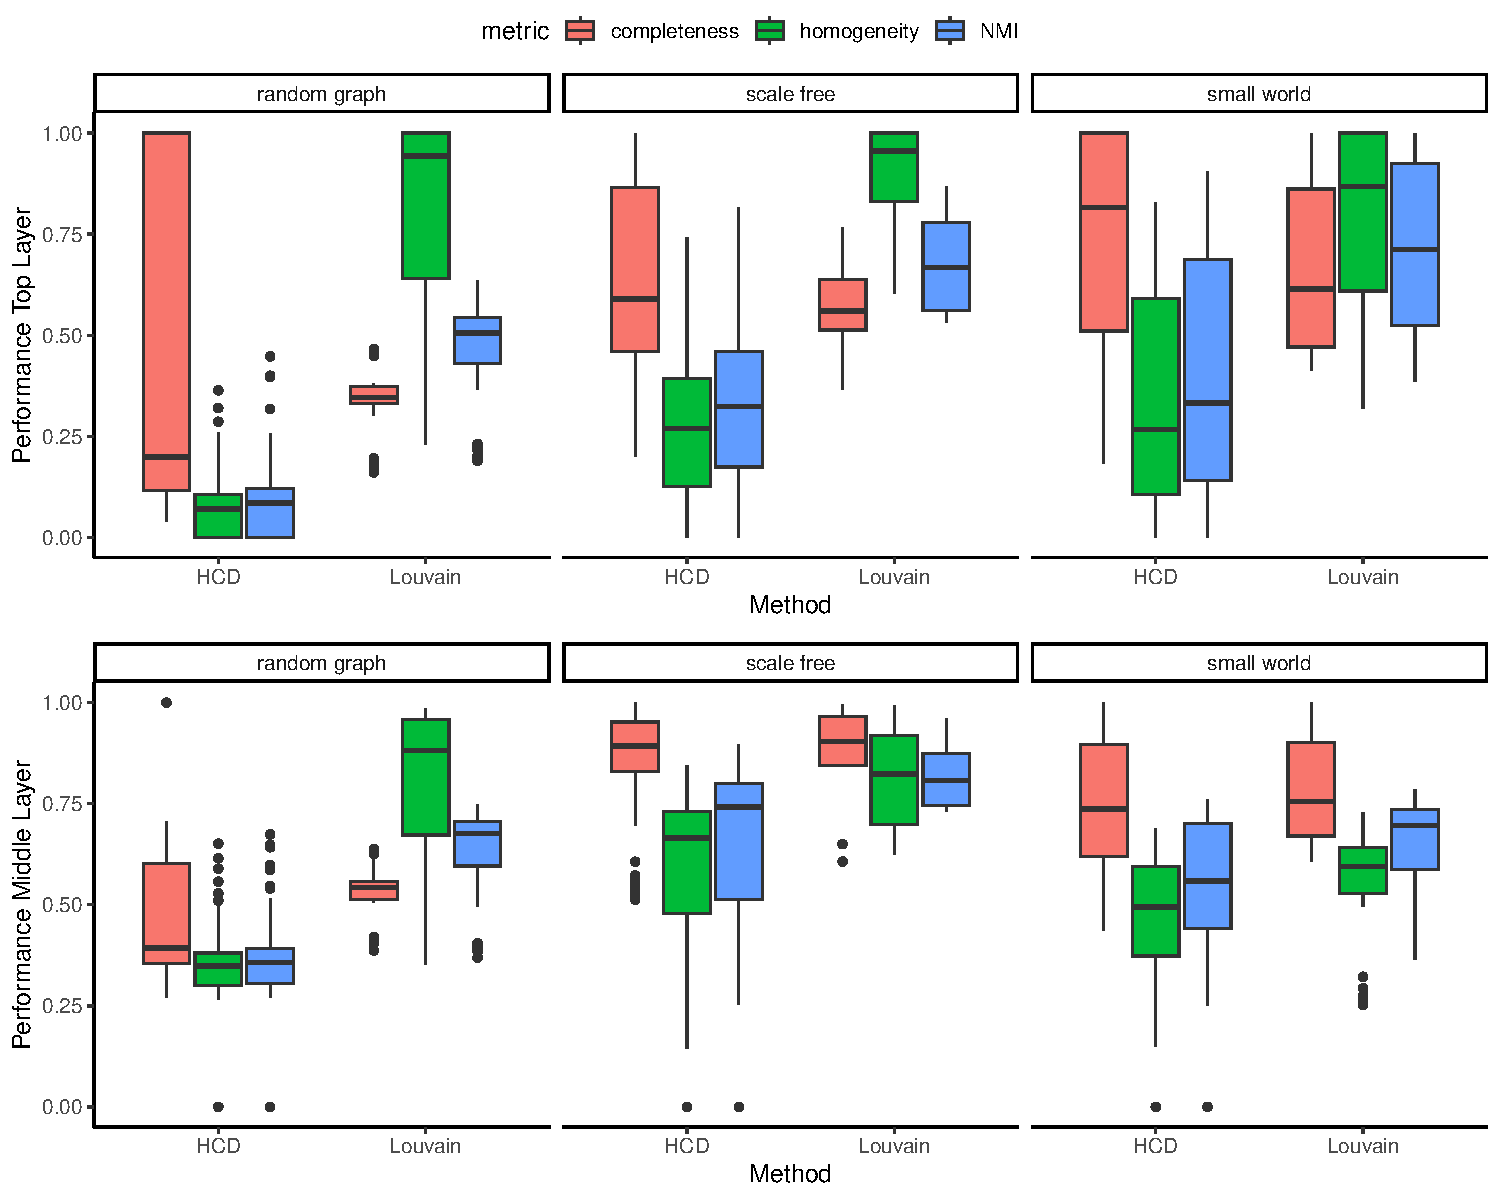
\includegraphics{Lab_report_4_1_2024_files/figure-latex/fig1-1.pdf}

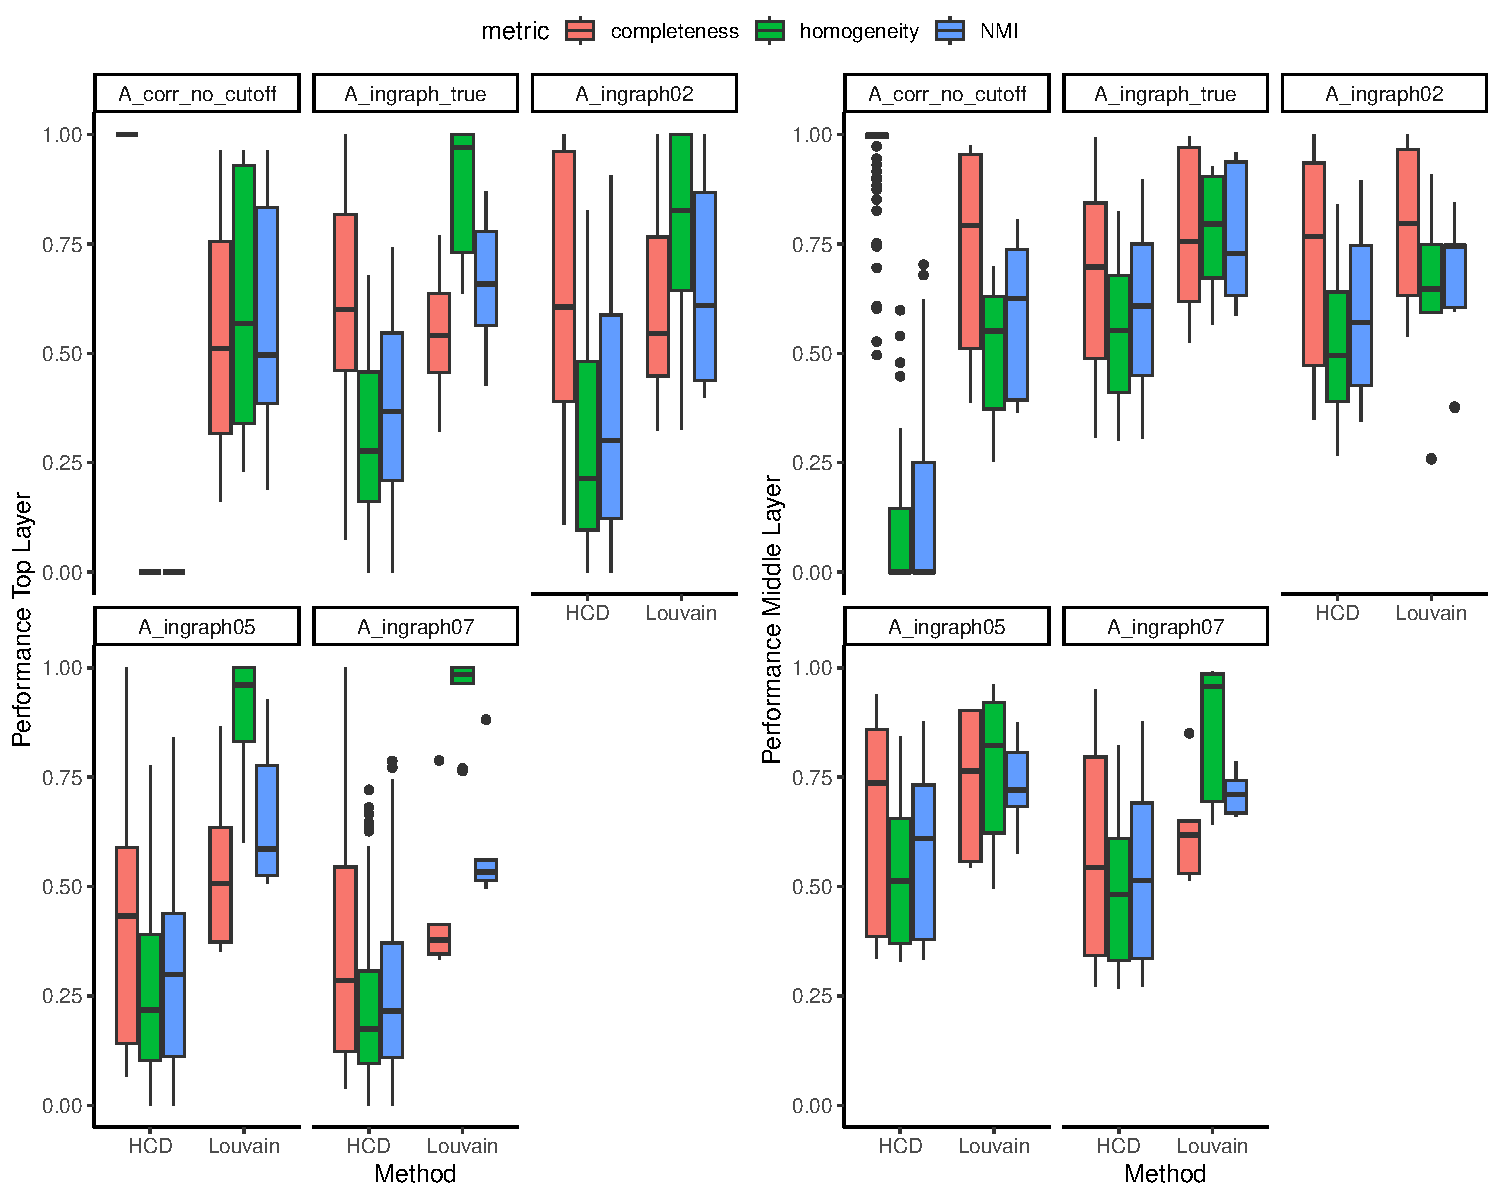
\includegraphics{Lab_report_4_1_2024_files/figure-latex/unnamed-chunk-7-1.pdf}

\begin{figure}
\centering
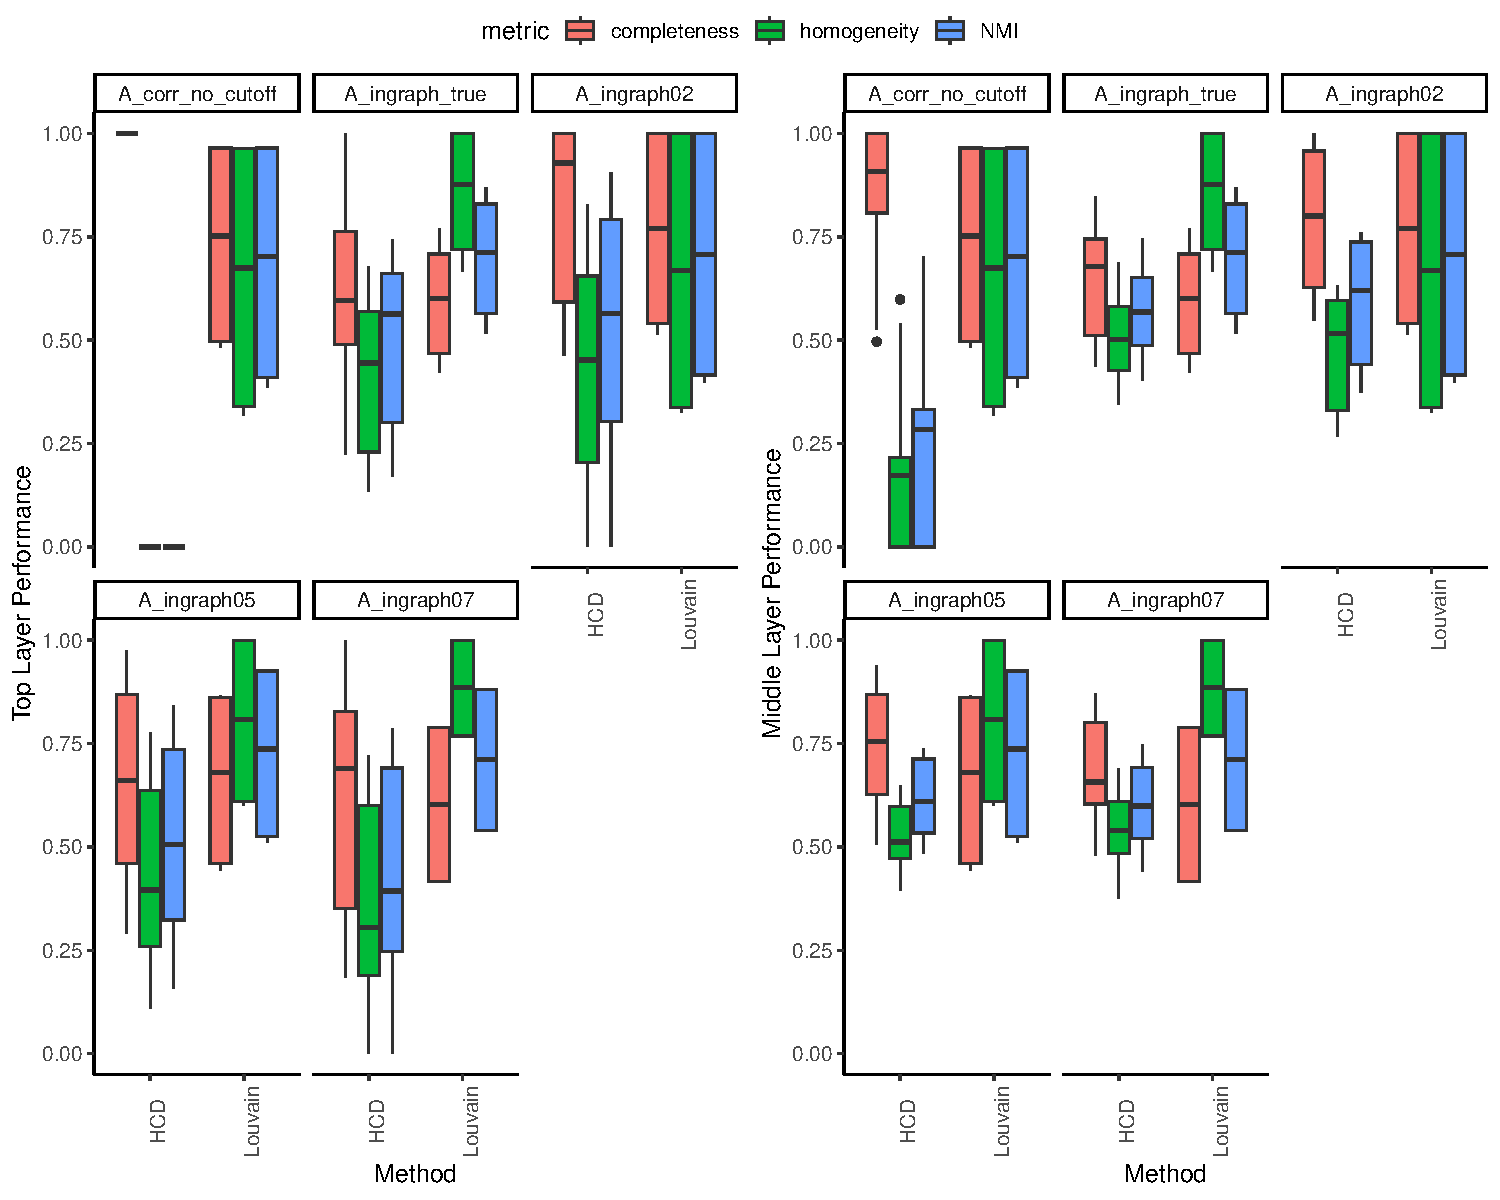
\includegraphics{Lab_report_4_1_2024_files/figure-latex/unnamed-chunk-8-1.pdf}
\caption{Small world graphs}
\end{figure}

\begin{figure}
\centering
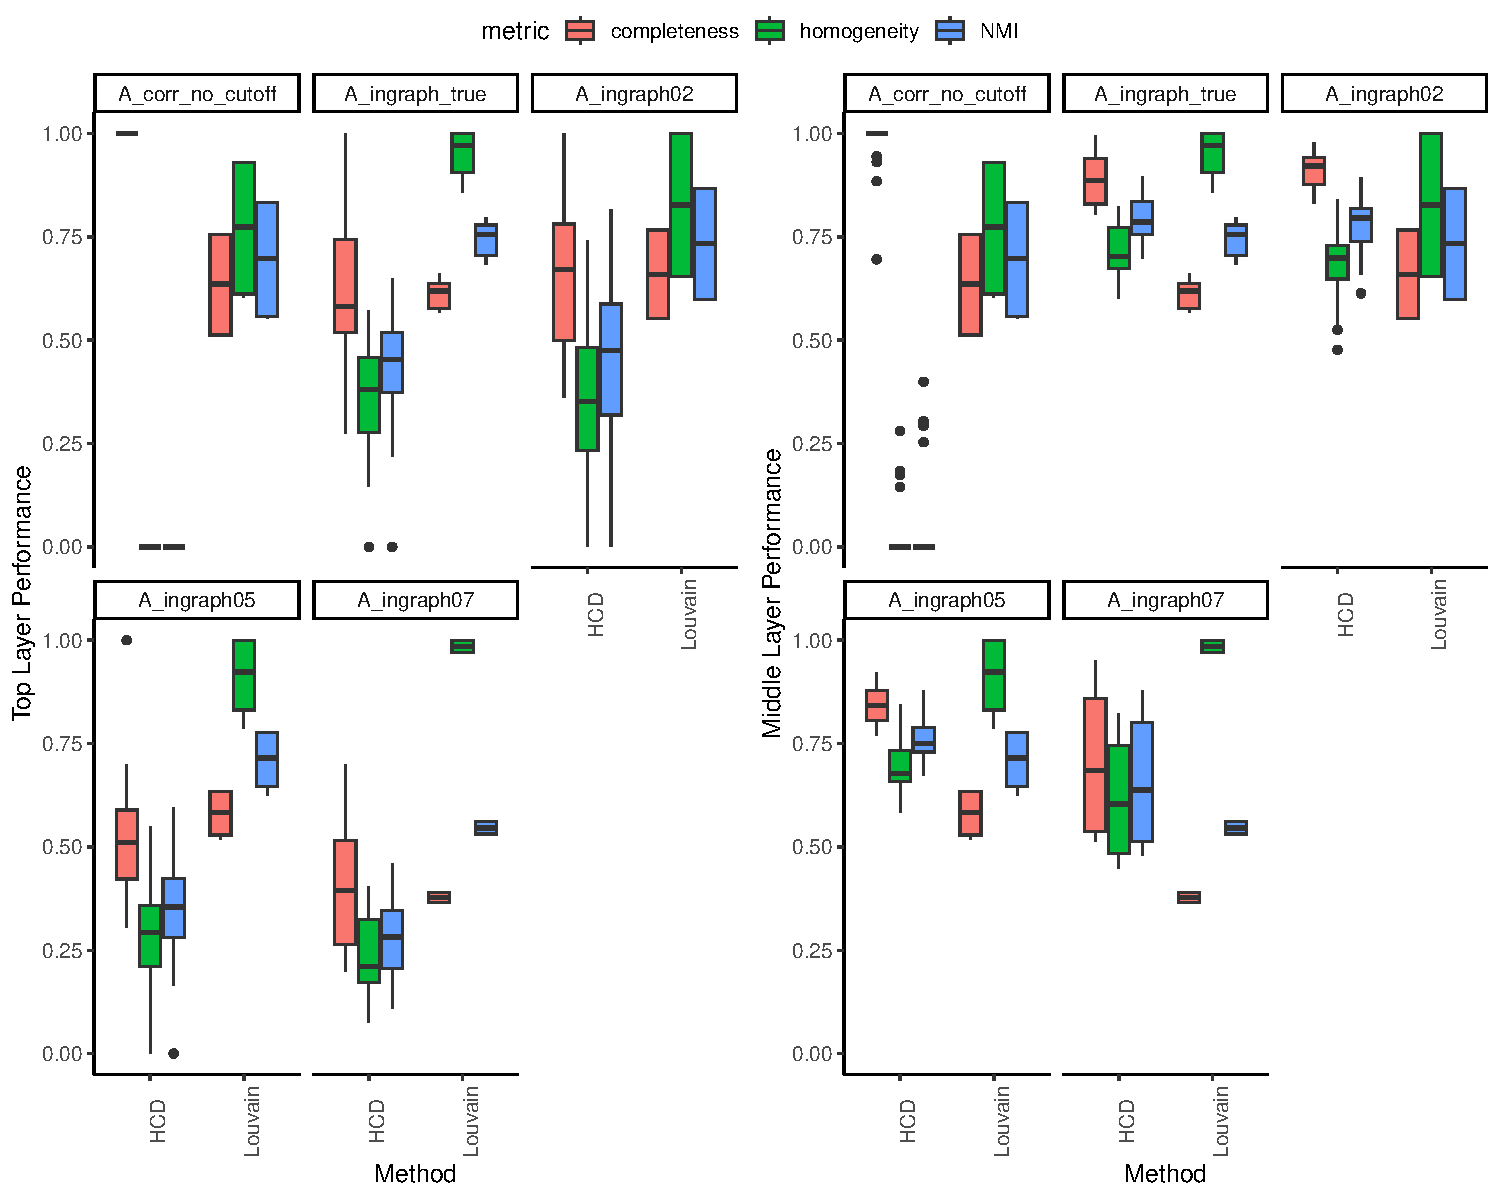
\includegraphics{Lab_report_4_1_2024_files/figure-latex/unnamed-chunk-9-1.pdf}
\caption{Scale free graphs}
\end{figure}

\begin{figure}
\centering
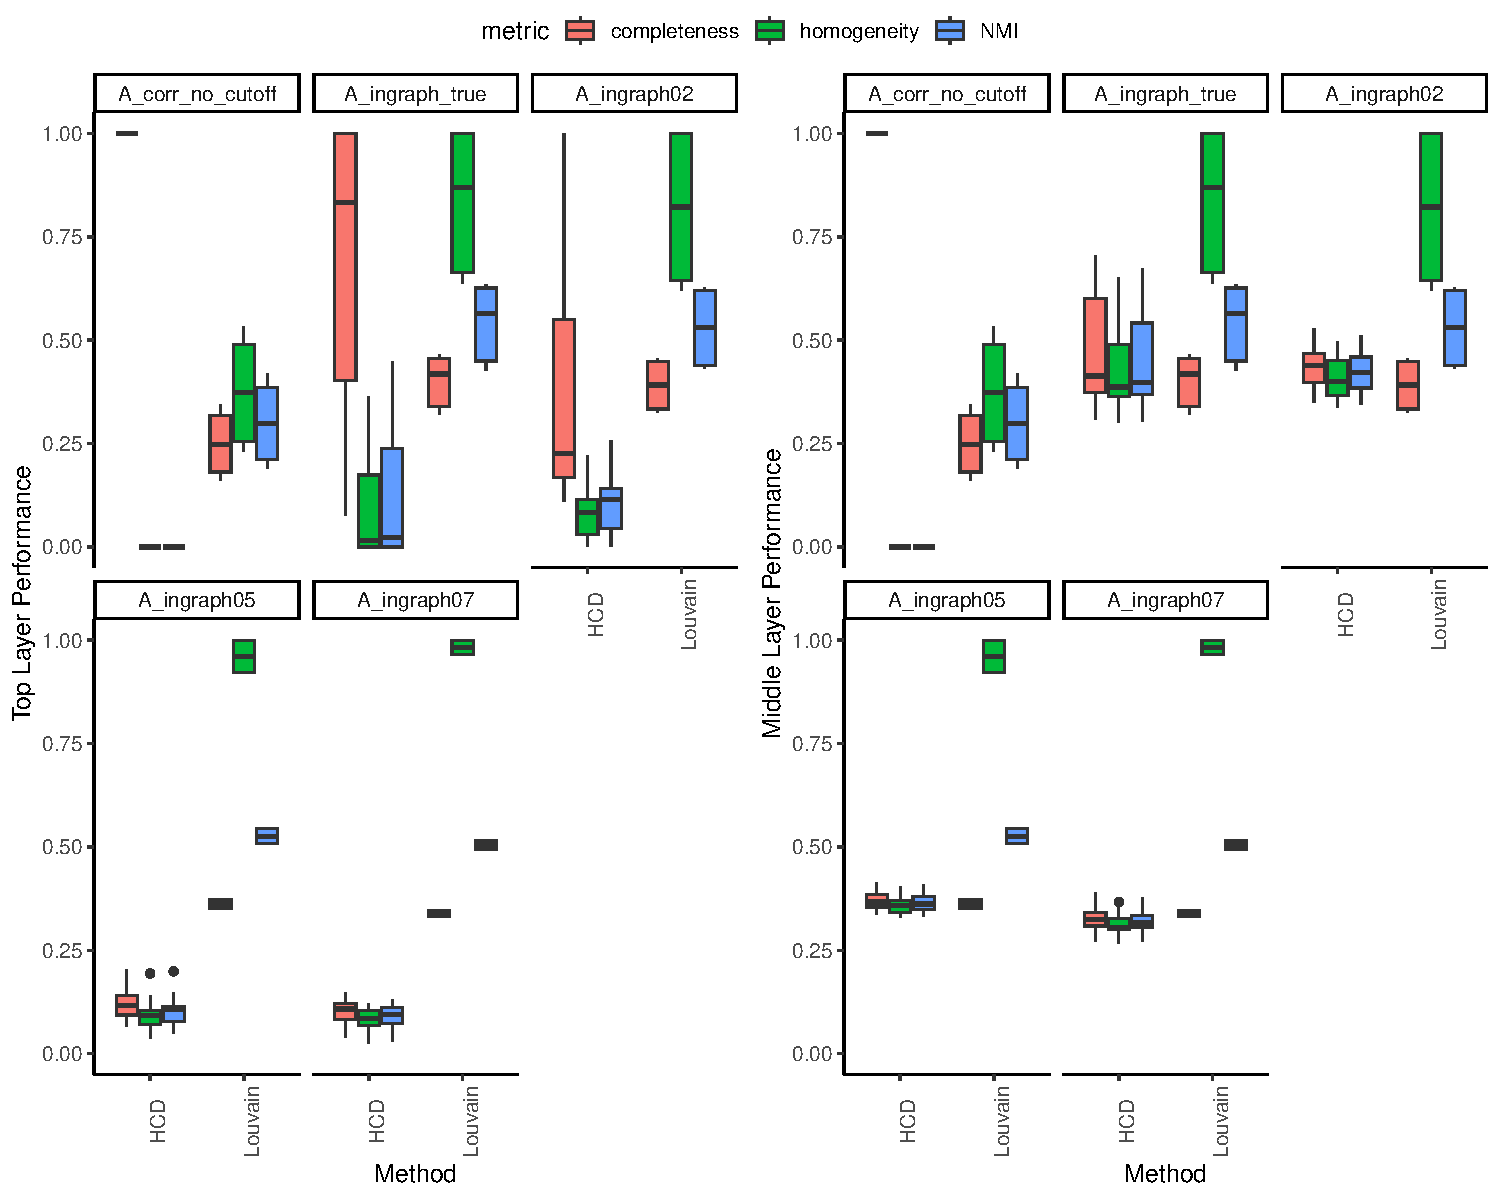
\includegraphics{Lab_report_4_1_2024_files/figure-latex/unnamed-chunk-10-1.pdf}
\caption{random graphs}
\end{figure}

\bibliographystyle{unsrt}
    \bibliography{C:/Users/Bruin/Desktop/Research Assistantship/Thesis Proposal Defense/proposal_references.bib}

\newpage
\section*{References}

\hypertarget{refs}{}
\begin{CSLReferences}{1}{0}
\leavevmode\vadjust pre{\hypertarget{ref-barabasi2003scale}{}}%
Barabási, Albert-László, and Eric Bonabeau. 2003. {``Scale-Free
Networks.''} \emph{Scientific American} 288 (5): 60--69.

\leavevmode\vadjust pre{\hypertarget{ref-watts1998collective}{}}%
Watts, Duncan J, and Steven H Strogatz. 1998. {``Collective Dynamics of
`Small-World'networks.''} \emph{Nature} 393 (6684): 440--42.

\end{CSLReferences}

\end{document}
